\chapter{Base de données et administration}
\label{ch-bdd-admin}


\section{Conception}

\subsection{Les démarches de conception}

\par Les Acteurs : un acteur représente l’abstraction d’un rôle joué par des entités externes. Dans notre application on distingue principalement deux acteurs qui sont les suivant :

\begin{itemize}
\item L'utilisateur qui peut écrire et compiler son code
\item L'administrateur qui possède les même droits que l'utilisateur mais possède aussi un accès à la page d'administration qui permet de modifier les tables Langages, Détails\_langages et Serveur (voir \ref{ss-partieApp})
\end{itemize}

\subsection{Modèle conceptuel des données (MCD)}
 
\par Le modèle conceptuel des données a pour but de définir de façon formelle la structure de la base de données qui sera utilisée par le système d'information. Il s'agit donc d'une représentation du modèle de données, facilement compréhensible, permettant de décrire le système d'informations à l'aide d'entités. 
La figure suivante présente le modèle conceptuel des données.

\begin{figure}[H]
\centering
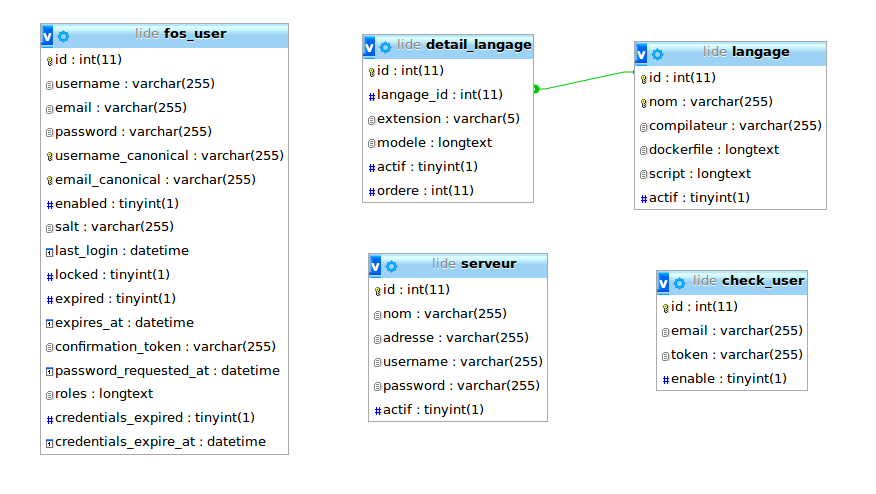
\includegraphics[width=0.8\textwidth]{./img/BDD.png}
\caption{Modèle conceptuel des données}
\end{figure}

\section{Base de données}

\subsection{Partie applicative}\label{ss-partieApp}

\par Les trois tables suivantes contiennent un champ actif qui permet d’activer ou de désactiver le tuple. Par exemple si un serveur est en maintenance ou ne doit pas être utilisé, il pourra être désactivé et réactivé au besoin par l’administrateur. C’est la même chose pour la table langage et details\_langage.


\subsubsection{Serveur}

\par La table Serveur permettra de connaître les serveurs disponibles. S'il y a une surcharge, l’administrateur aura juste à ajouter un nouveau serveur et l’application pourra directement l’utiliser si besoin.

\subsubsection{Langage}

\par Le nom d’un langage est UNIQUE. La table Langage contient le Dockerfile permettant d’installer le nécessaire pour pouvoir compiler/exécuter le langage. Il y a aussi le script qui permet de lancer la compilation avec les fichiers de l’utilisateur ainsi que le compilateur. 
L’avantage de stocker en base de données les langages est de rendre autonome les enseignants. S’ils veulent rajouter un nouveau langage, il leur suffit de l’ajouter avec son Dockerfile et son script.

\subsubsection{Détails langage}

\par La table details\_langage contient les extensions du langage correspondant ainsi qu’un modèle de base (par exemple le Hello World). Cela permet de proposer à l’utilisateur l’extension qu’il veut écrire.

\subsection{Partie administration}

\subsubsection{Fos user}

\par Dans cette table, on sauvegarde tous les informations des utilisateurs.

\subsubsection{Check\_user}

Cette table a pour but de sauvegarder les e-mails des utilisateurs qui n’ont pas encore confirmé leur inscription via le lien de validation reçu dans leur boite mail. 

\section{Administration}

\par Pour mettre en place l’interface administrateur, nous avons utilisé différents outils proposé par Symfony et notamment les bundles FOSUserBundle et EasyAdminBundle.

\subsection{FOSUserBundle}

\par FOSUserBundle est un bundle qui fournit un système de gestion des utilisateurs complet. \\

\par Ce système comprend notamment :

\begin{itemize}
	\item Un formulaire d’inscription avec e-mail de confirmation pour vérifier l'authenticité de l’adresse fournie par l'utilisateur
	\item Un système de récupération de mot de passe (de type <<mot de passe oublié?>>)
	\item Une compatibilité avec la librairie Doctrine pour le stockage en Base de données

\end{itemize}

\par Ces différentes fonctionnalités nous ont permet de sécuriser l’accès à l’application et aussi de paramétrer les droits d’accès à certaines ressources en attribuant des rôles.


\subsection{EasyAdminBundle}

\par Ce bundle nous a permis de créer facilement l’interface administrateur en générant automatiquement les différents formulaires associés aux entités, telles que User et Langage. Il fournit aussi la possibilité d’appliquer les opérations CRUD\footnote{Create, Read, Update, Delete} sur les différentes entités.

\par Doctrine permet de créer des objets (entités) pour gérer les fux entrants et sortants vers la base de données. Ces entités gèrent également le côté relationnel des données. L’ORM Doctrine possède divers commandes permettant la génération automatique des entités. Néanmoins, cette génération reste très basique et il est nécessaire de les modifier afin d’ajouter les relations inter-entités (clé étrangère, relation multidirectionnelle ...) 

\par Les différentes requêtes SQL sont définies sous forme de fonctions dans les fichiers entités, ce qui permet de sécuriser l’appel à ces dernières depuis les contrôleurs.